\section{Experiments and Results}
\label{sec:experiments}
In this section, we present the experimental setup, results, and analysis of the \textit{EnCoMP} framework. We evaluate the performance of \textit{EnCoMP} in real-world outdoor test scenarios that are not part of the original training dataset and compare it with state-of-the-art baselines.


\subsection{Evaluation Metrics}
We evaluate the performance of \textit{EnCoMP} and the baselines using the following metrics:

\begin{itemize}
\item \textbf{Success Rate}: The percentage of trials in which the robot successfully reaches the goal location without being detected by threats, colliding with obstacles, or running out of time.
\item \textbf{Navigation Time}: The average time taken by the robot to navigate from the start position to the goal location in successful trials.
\item \textbf{Trajectory Length}: The average length of the path traversed by the robot from the start position to the goal location in successful trials.

\item \textbf{Threat Exposure}: The average percentage of time the robot is exposed to threats during navigation, calculated as the ratio of the time spent in the line-of-sight of threats to the total navigation time.
\item \textbf{Cover Utilization}: The average percentage of time the robot utilizes cover objects during navigation, calculated as the ratio of the time spent in high cover density areas (as indicated by the cover map) to the total navigation time.
\end{itemize}



\subsection{Baselines}
We compare the performance of \textit{EnCoMP} against the following state-of-the-art navigation methods:
\begin{itemize}

   \item \textbf{CoverNav:} A deep reinforcement learning-based system designed for navigation planning that prioritizes the use of natural cover in unstructured outdoor environments. This strategy aims to enhance stealth and safety in potentially hostile settings ~\cite{hossain2023covernav}.
    
    \item \textbf{VAPOR:} A method for autonomous legged robot navigation in unstructured, densely vegetated outdoor environments using offline reinforcement learning ~\cite{weerakoon2023vapor}.
    
    \item \textbf{VERN:} An approach for vegetation-aware robot navigation, which facilitates efficient traversal in densely vegetated and unstructured outdoor environments. Their method integrates sensory data and learning algorithms to navigate with an understanding of vegetation density and type ~\cite{sathyamoorthy2023vern}.
\end{itemize}


\subsection{Implementation Details}
Our offline RL network is implemented in PyTorch and trained in a workstation with a 10th-generation Intel Core i9-10850K processor and an NVIDIA GeForce RTX 3090 GPU. For real-time deployment and inference, we use the Jackal UGV from Clearpath Robotics which runs on the Robot Operating System (ROS) Noetic distribution. The Jackal UGV is equipped with a 3D VLP-32C Velodyne Ultrapuck LiDAR,  an AXIS Fixed IP camera, featuring a fixed-focus lens with 30 fps/VGA resolution. The system’s processing capabilities are powered by an onboard Intel computer system, equipped with an Intel i7-9700TE CPU and an NVIDIA GeForce GTX 1650 Ti GPU.


The CQL algorithm is configured with a learning rate of \(1 \times 10^{-4}\), a batch size of 256, and a discount factor \(\gamma = 0.95\). The regularization term weight \(\alpha\) is set to 0.2 to balance exploration and exploitation. The neural networks used in the CQL algorithm employ ReLU activation functions for the hidden layers and a linear activation for the output layer. These hyperparameters were fine-tuned through extensive experimentation to optimize learning efficiency and ensure robust performance in covert navigation tasks.
The training process was conducted over 500 episodes to ensure stable convergence and robust performance of the learned policy.

To ensure safe navigation and obstacle avoidance, we also integrate the Dynamic Window Approach (DWA) ~\cite{fox1997dynamic} into the \textit{EnCoMP} framework. DWA is a local planner that generates velocity commands for the robot based on the current sensor readings and the robot's dynamics. It optimizes the velocity commands by considering the robot's current velocity, the obstacles in the environment, and the goal location.

% \subsection{Experimental Parameters and Settings}
% We provide detailed information on the experimental parameters and settings used in our evaluation:

% \begin{itemize}
% \item \textbf{Reward Weights:} The reward function weights were carefully tuned to balance the various objectives of the covert navigation task. Specifically, $\lambda_c = 0.5$ for the cover utilization reward, $\lambda_t = 1.5$ for the threat exposure penalty, $\lambda_g = 1.0$ for the goal-reaching reward, and $\lambda_o = 5.0$ for the collision avoidance penalty. These weight values were determined through extensive empirical evaluation to ensure effective and safe navigation while prioritizing threat avoidance and goal-reaching efficiency over cover utilization.
% \item \textbf{CQL Hyperparameters:} The Conservative Q-Learning (CQL) algorithm was configured with a learning rate of $1 \times 10^{-4}$, a batch size of 256, and a discount factor $\gamma = 0.95$. To achieve a balance between exploration and exploitation, the regularization term weight $\alpha$ was set to 0.2. The neural networks employed ReLU activation functions for the hidden layers and a linear activation for the output layer. These hyperparameter values were subsequently fine-tuned through extensive experimentation to optimize learning efficiency and ensure robust performance in our covert navigation tasks. The training process was conducted over 1,000 episodes to ensure stable convergence and robust performance of the learned policy
% \end{itemize}



\subsection{Testing Scenarios}
\label{sec:testingscenario}
We evaluate our covert-based navigation framework in three diverse outdoor environments. The three testing scenarios present increasing levels of difficulty for covert navigation:
% We evaluate our covert-based navigation framework in three diverse outdoor environments (see Fig. \ref{fig:environments_maps}):

\begin{itemize}
\item \textbf{Scenario 1}: An urban environment with buildings, structures, and sparse vegetation.
\item \textbf{Scenario 2}: A densely vegetated forest environment with trees, bushes, and uneven terrain.
\item \textbf{Scenario 3}: A mixed environment with both urban structures and natural vegetation.
\end{itemize}

Each scenario presents unique challenges for covert navigation, such as varying levels of cover availability, threat exposure, and terrain complexity.
\subsection{Performance Comparison and Analysis}
Table \ref{tab:real_results} demonstrates \textit{EnCoMP}'s significant improvements over existing navigation systems across all evaluation metrics and testing scenarios. Each scenario was tested with at least 10 runs to ensure the consistency and reliability of the results. In terms of success rate, \textit{EnCoMP} consistently outperforms the baseline methods across all scenarios, achieving success rates of 95\%, 93\%, and 91\% in Scenarios 1, 2, and 3, respectively. This demonstrates the effectiveness of our approach in navigating complex environments while maintaining covertness and avoiding threats. \textit{EnCoMP} also exhibits the shortest navigation times and trajectory lengths compared to the baselines, indicating its efficiency in reaching the goal location. The reduced navigation times and trajectory lengths can be attributed to the informed decision-making enabled by the multi-modal perception pipeline and the learned covert navigation policy. Our approach achieves the highest exploration coverage percentages, demonstrating its ability to thoroughly explore the environment while navigating towards the goal. The high exploration coverage ensures that the robot can identify potential cover locations and threats more effectively.

Notably, \textit{EnCoMP} significantly reduces the threat exposure percentage compared to the baselines, with values of 10.5\%, 12.0\%, and 14.5\% in Scenarios 1, 2, and 3, respectively. This highlights the effectiveness of our approach in minimizing the robot's visibility to threats and maintaining a high level of covertness during navigation. Furthermore, \textit{EnCoMP} achieves the highest cover utilization percentages, indicating its ability to effectively leverage the available cover objects in the environment. By actively seeking and utilizing cover, our approach enhances the robot's survivability and reduces the risk of detection. 

Fig. \ref{fig:trajectories} presents sample navigation trajectories generated by \textit{EnCoMP} and the baseline methods in the three testing scenarios. As evident from the trajectories, \textit{EnCoMP} generates paths that prioritize cover utilization and threat avoidance, while the baseline methods often result in more exposed and less efficient paths. Also, to illustrate the effectiveness of \textit{EnCoMP} in generating safer paths and minimizing exposure to high-threat regions, we present a visualization (Figure~\ref{fig:threat_map_visualization}) of the threat map and the trajectories generated by \textit{EnCoMP} and CoverNav \cite{hossain2023covernav} in a representative scenario.

\begin{figure*}[!htb]
    \centering
    \subfloat[\centering]{{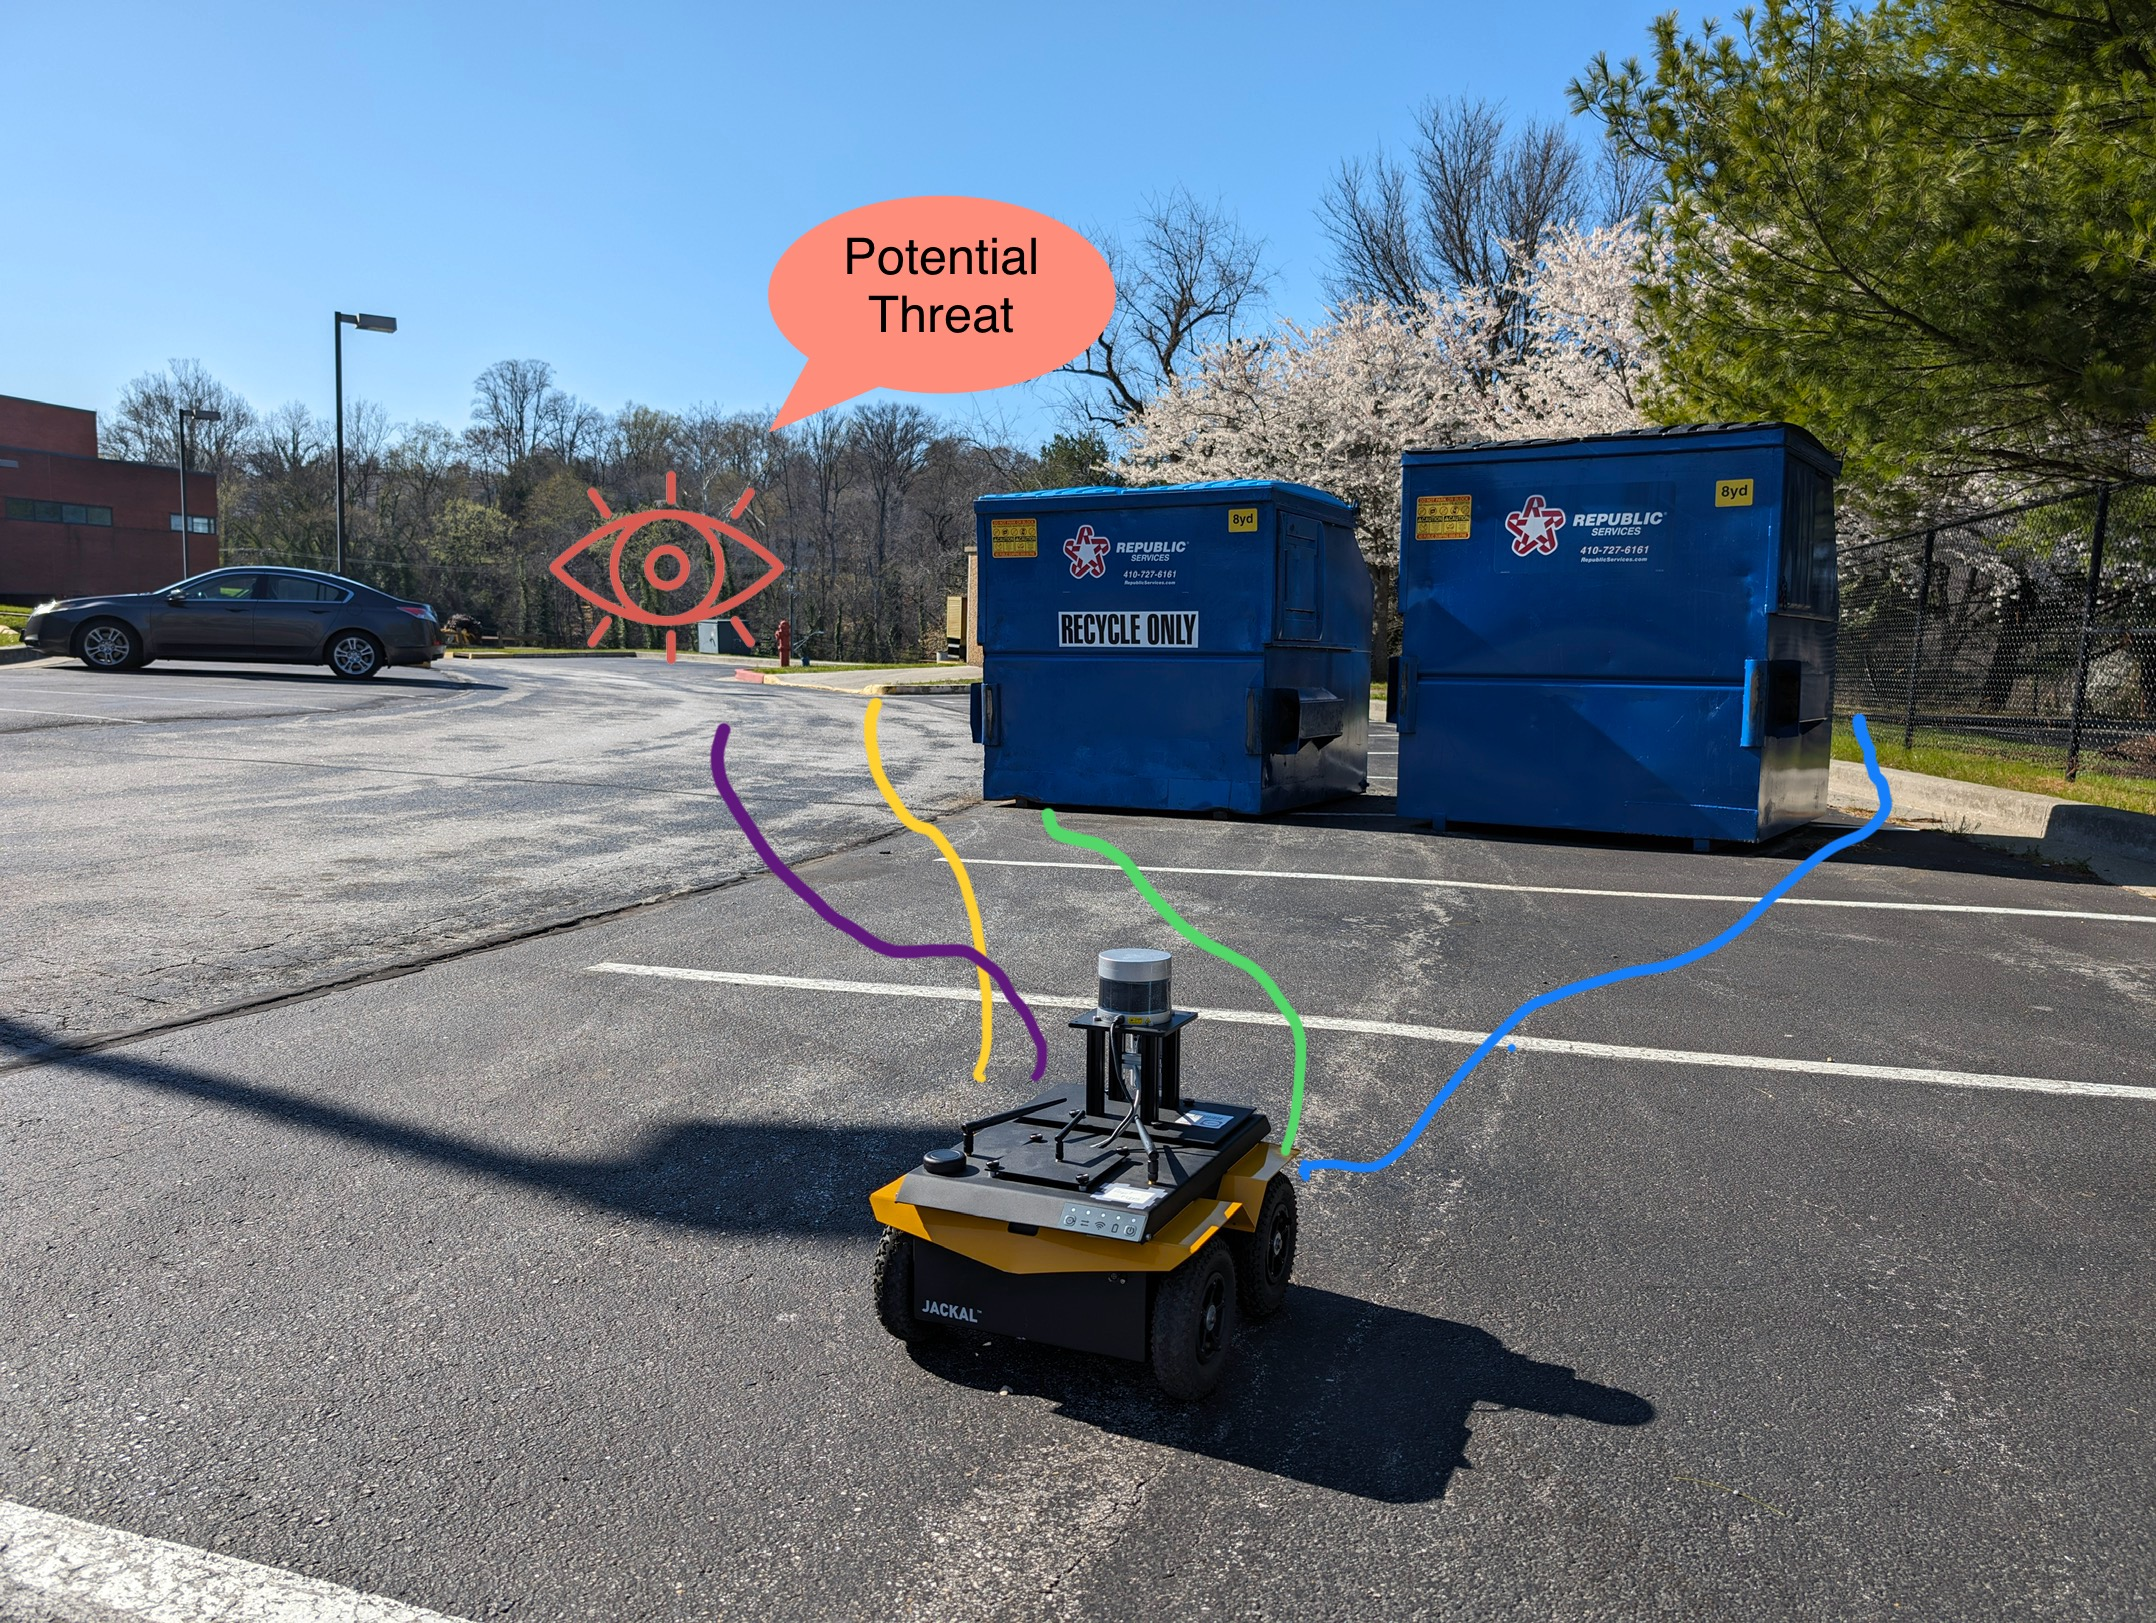
\includegraphics[width=.31\textwidth]{sections/images/scenario_1_2.jpeg}}}%
    \quad % Adjusted for more uniform spacing
    \subfloat[\centering ]{{\includegraphics[width=.31\textwidth]{sections/images/scenario_2_2.jpeg} }}%
    \quad % Adjusted for more uniform spacing
    \subfloat[\centering]{{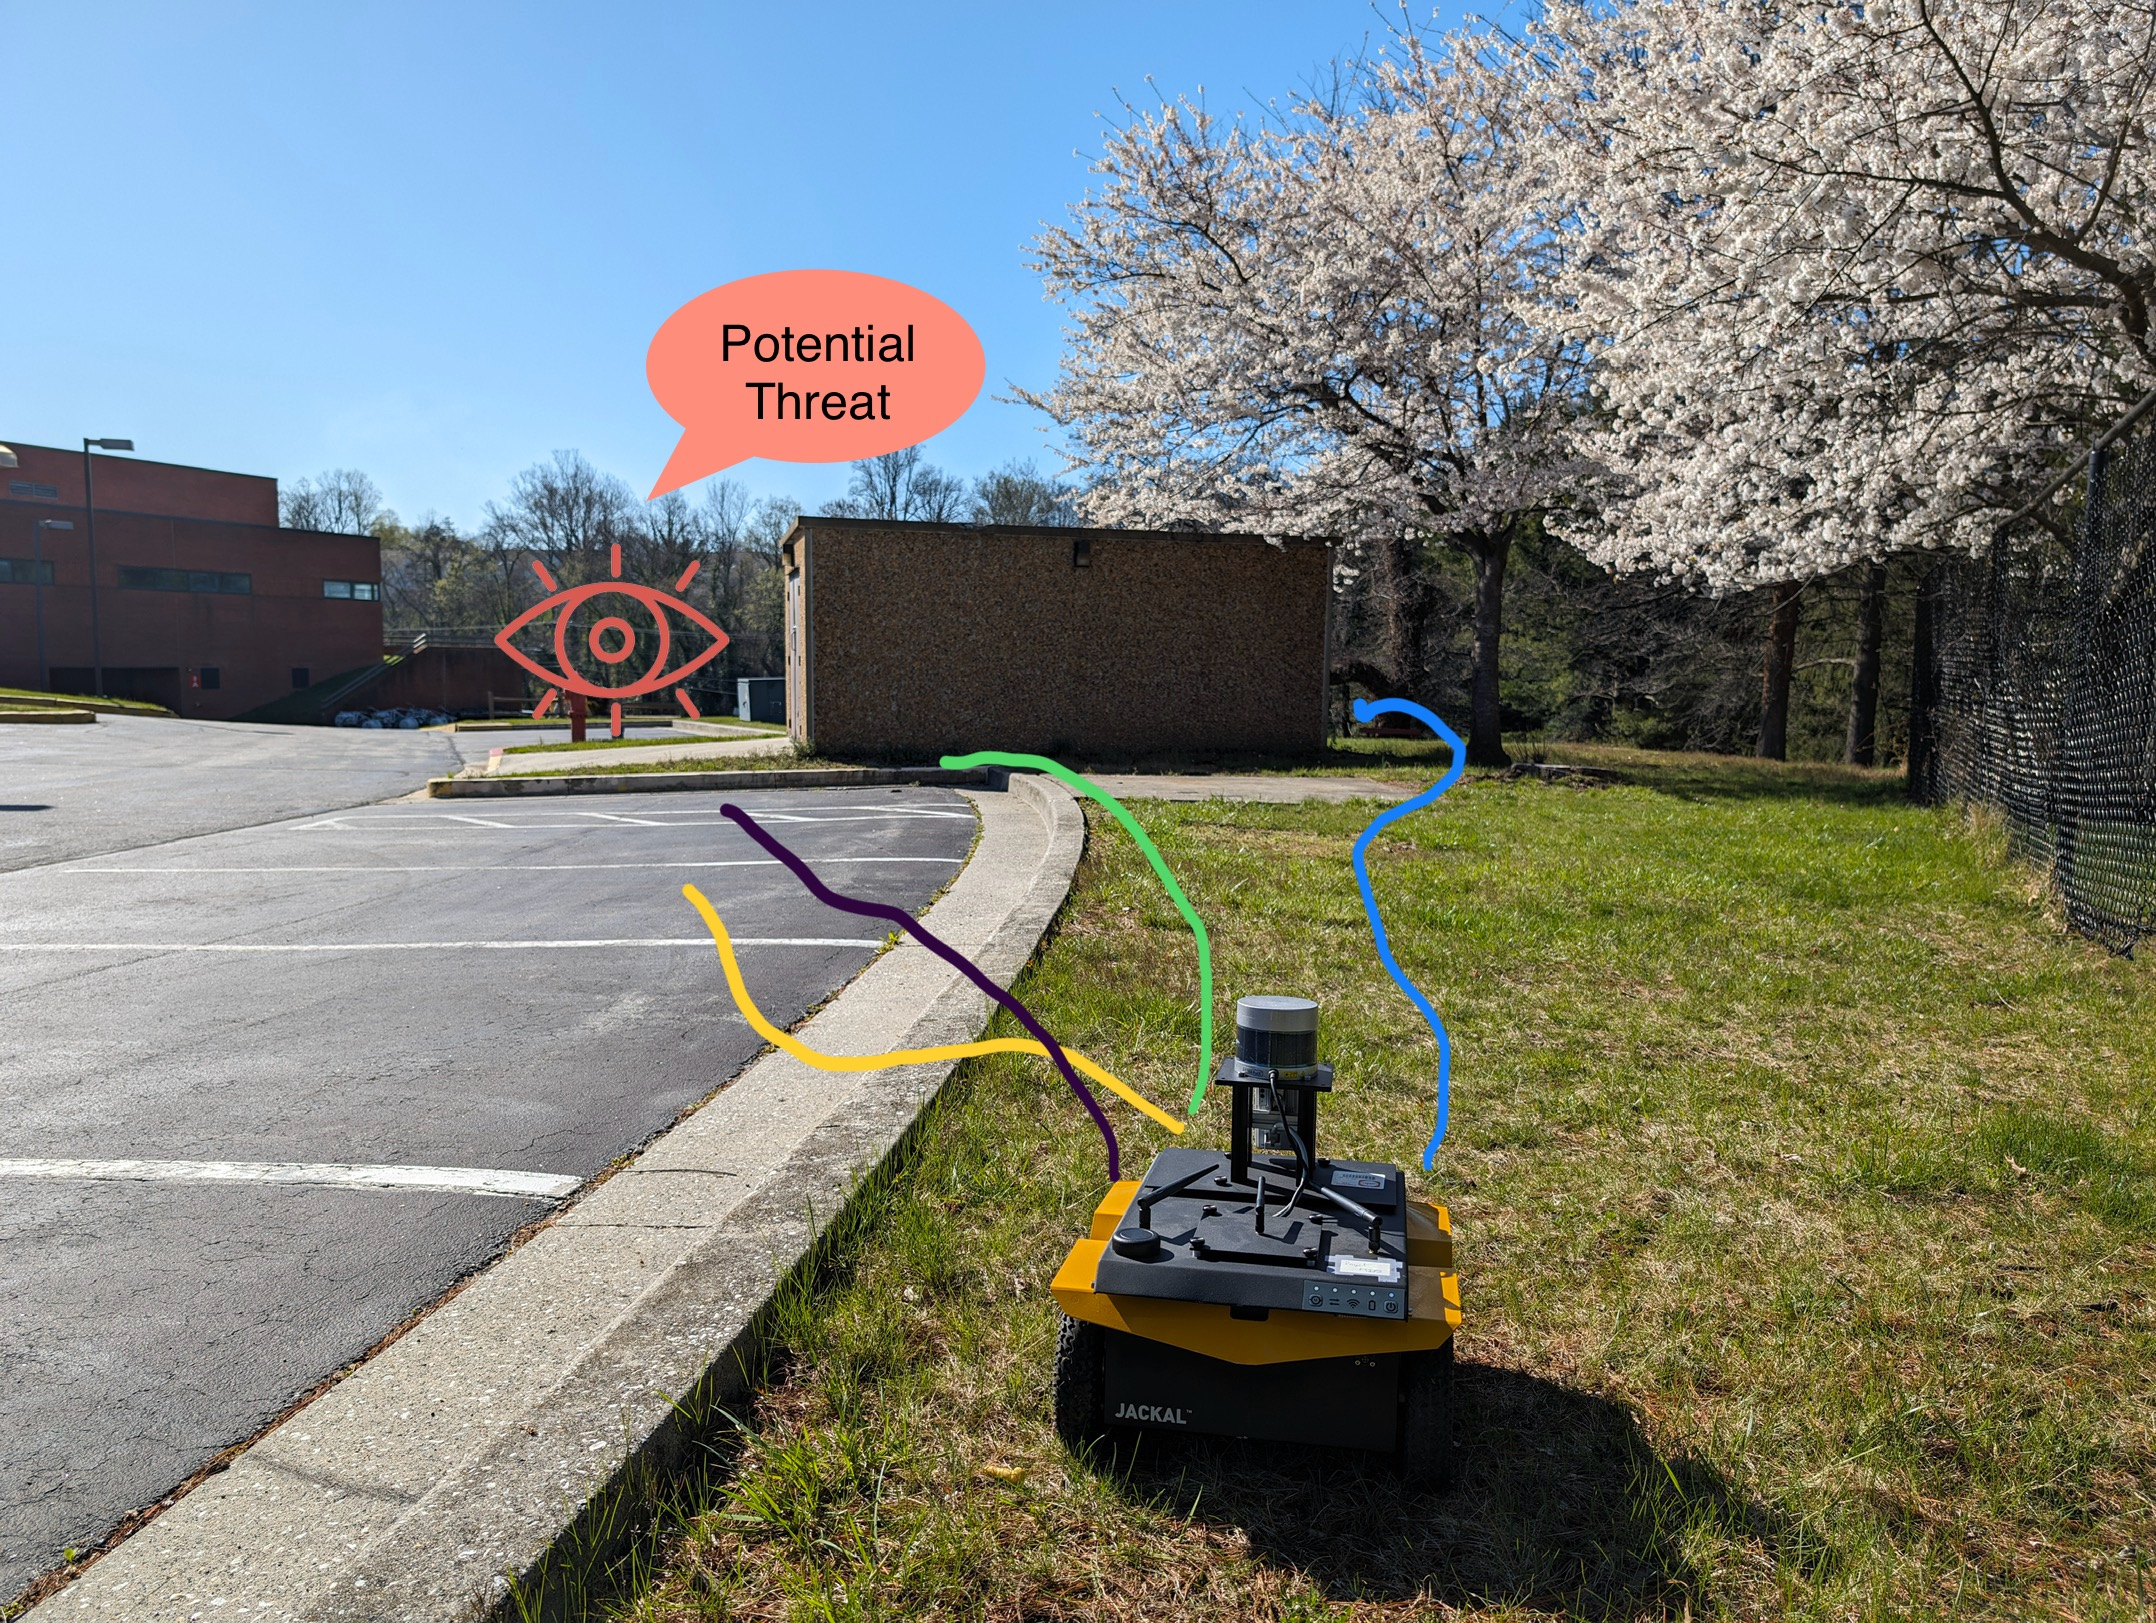
\includegraphics[width=.31\textwidth]{sections/images/scenario_3_3.jpeg}}}%
    
    \caption{Comparison of navigation strategies in diverse outdoor settings (See \ref{sec:testingscenario}). (a) Scenario 1, (b) Scenario 2, (c) Scenario 3. Paths indicate the trajectories taken by different systems, with \textit{EnCoMP} (blue) demonstrating more optimized routes that effectively leverage cover while minimizing threat exposure, in contrast to CoverNav (green), VAPOR (purple), and VERN (yellow).}%
    \label{fig:trajectories}
\end{figure*}

% \begin{table}[ht]
% \centering
% \scriptsize
% \begin{tabular}{|l|c|c|c|c|}
% \hline
% \textbf{Metrics} & \textbf{Methods} & \textbf{Scen. 1} & \textbf{Scen. 2} & \textbf{Scen. 3} \\
% \hline
% \textbf{Success} & CoverNav & 85 & 83 & 81 \\
% \textbf{Rate (\%)}& VAPOR & 87 & 85 & 84 \\
% & VERN & 88 & 86 & 85 \\
% & \textbf{EnCoMP(Ours)} & \textbf{95} & \textbf{93} & \textbf{91} \\
% \hline
% \textbf{Navigation} & CoverNav & 40.0 & 42.5 & 45.0 \\
% \textbf{Time (s)} & VAPOR & 38.5 & 40.0 & 42.0 \\
% & VERN & 39.0 & 41.0 & 43.5 \\
% & \textbf{EnCoMP(Ours)} & \textbf{32.0} & \textbf{34.5} & \textbf{36.0} \\
% \hline
% \textbf{Trajectory} & CoverNav & 14.0 & 14.5 & 15.0 \\
% \textbf{Length (m)} & VAPOR & 13.5 & 14.0 & 14.5 \\
% & VERN & 13.8 & 14.3 & 14.8 \\
% & \textbf{EnCoMP(Ours)} & \textbf{11.0} & \textbf{12.0} & \textbf{12.5} \\
% \hline
% \textbf{Threat} & CoverNav & 22.5 & 25.0 & 27.5 \\
% \textbf{Exposure (\%)} & VAPOR & 20.0 & 22.5 & 25.0 \\
% & VERN & 18.5 & 21.0 & 23.5 \\
% & \textbf{EnCoMP(Ours)} & \textbf{10.5} & \textbf{12.0} & \textbf{14.5} \\
% \hline
% \textbf{Cover} & CoverNav & 65.0 & 62.5 & 60.0 \\
% \textbf{Utilization (\%)} & VAPOR & 67.5 & 65.0 & 62.5 \\
% & VERN & 70.0 & 67.5 & 65.0 \\
% & \textbf{EnCoMP(Ours)} & \textbf{85.0} & \textbf{82.5} & \textbf{80.0} \\
% \hline
% \end{tabular}
% \caption{Comparative Analysis: \textit{EnCoMP} vs. SOTA methods across three scenarios, highlighting superior performance in metrics such as success rate, navigation time, threat exposure, and cover utilization.}
% \label{tab:real_results}
% \end{table}


\begin{table}[ht]
\centering
\scriptsize
\begin{tabular}{|l|c|c|c|c|}
\hline
\textbf{Metrics} & \textbf{Methods} & \textbf{Scen. 1} & \textbf{Scen. 2} & \textbf{Scen. 3} \\
\hline
\textbf{Success} & CoverNav & 85 & 83 & 81 \\
\textbf{Rate (\%)} & VAPOR & 87 & 85 & 84 \\
& VERN & 88 & 86 & 85 \\
& EnCoMP w/o ATAVE & 90 & 88 & 86 \\
& \textbf{EnCoMP(Ours)} & \textbf{95} & \textbf{93} & \textbf{91} \\
\hline
\textbf{Navigation} & CoverNav & 40.0 & 42.5 & 45.0 \\
\textbf{Time (s)} & VAPOR & 38.5 & 40.0 & 42.0 \\
& VERN & 39.0 & 41.0 & 43.5 \\
& EnCoMP w/o ATAVE & 35.0 & 37.5 & 40.0 \\
& \textbf{EnCoMP(Ours)} & \textbf{32.0} & \textbf{34.5} & \textbf{36.0} \\
\hline
\textbf{Trajectory} & CoverNav & 14.0 & 14.5 & 15.0 \\
\textbf{Length (m)} & VAPOR & 13.5 & 14.0 & 14.5 \\
& VERN & 13.8 & 14.3 & 14.8 \\
& EnCoMP w/o ATAVE & 12.5 & 13.0 & 13.5 \\
& \textbf{EnCoMP(Ours)} & \textbf{11.0} & \textbf{12.0} & \textbf{12.5} \\
\hline
\textbf{Threat} & CoverNav & 22.5 & 25.0 & 27.5 \\
\textbf{Exposure (\%)} & VAPOR & 20.0 & 22.5 & 25.0 \\
& VERN & 18.5 & 21.0 & 23.5 \\
& EnCoMP w/o ATAVE & 15.0 & 17.5 & 20.0 \\
& \textbf{EnCoMP(Ours)} & \textbf{10.5} & \textbf{12.0} & \textbf{14.5} \\
\hline
\textbf{Cover} & CoverNav & 65.0 & 62.5 & 60.0 \\
\textbf{Utilization (\%)} & VAPOR & 67.5 & 65.0 & 62.5 \\
& VERN & 70.0 & 67.5 & 65.0 \\
& EnCoMP w/o ATAVE & 75.0 & 72.5 & 70.0 \\
& \textbf{EnCoMP(Ours)} & \textbf{85.0} & \textbf{82.5} & \textbf{80.0} \\
\hline
\end{tabular}
\caption{Comparative Analysis: \textit{EnCoMP} vs. SOTA methods across three scenarios, highlighting superior performance in metrics such as success rate, navigation time, threat exposure, and cover utilization.}
\label{tab:real_results}
\end{table}

\begin{figure}[!htb]
    \centering
    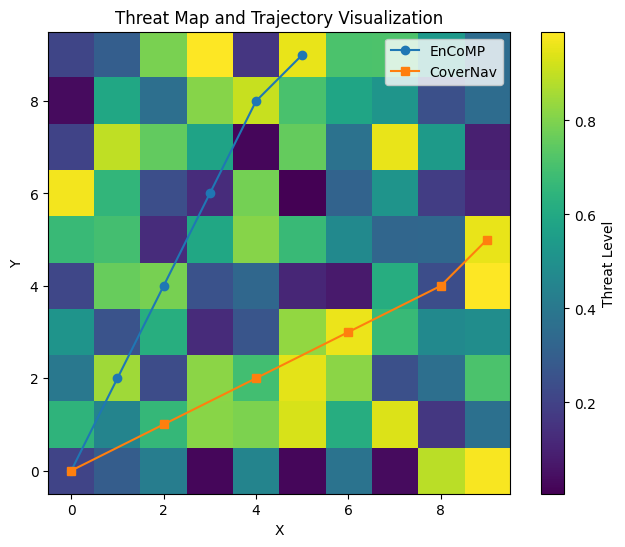
\includegraphics[width=\linewidth]{sections/images/threat_map_visualization.png}
    \caption{ A visualization of the threat map and the trajectories generated by \textit{EnCoMP} and CoverNav ~\cite{hossain2023covernav} in a representative scenario. The threat map, depicted by the colormap, indicates the level of threat associated with different locations in the environment, with darker colors representing higher threat levels. The \textit{EnCoMP} trajectory (orange line with circular markers) navigates through regions with lower threat levels, demonstrating its ability to identify and prioritize safer routes. In contrast, the CoverNav trajectory (blue line with square markers) traverses through areas with higher threat levels, suggesting a less effective threat avoidance capability. This visualization highlights \textit{EnCoMP}'s superior performance in generating safer paths and minimizing exposure to high-threat regions compared to CoverNav.}
   \label{fig:threat_map_visualization}
\end{figure}

\textbf{Ablation Study for the ATAVE Algorithm:}
We conduct an ablation study to evaluate the impact of the Adaptive Threat-Aware Visibility Estimation (ATAVE) algorithm on the navigation performance of \textit{EnCoMP}. We compare two variants of \textit{EnCoMP}: one with ATAVE and one without ATAVE. The variant without ATAVE relies solely on the cover map and height map for navigation, selecting waypoints based on the highest cover density and lowest elevation. In contrast, \textit{EnCoMP} with ATAVE incorporates dynamic threat assessment and adaptive visibility estimation to generate safer and more efficient trajectories (see Figure \ref{fig:threat_map_visualization}). By considering the potential threats and their visibility, ATAVE enhances the robot's situational awareness and enables it to make informed decisions during covert navigation. The ablation study demonstrates the significant contribution of ATAVE to \textit{EnCoMP}'s overall performance, resulting in higher success rates, lower threat exposure, and improved cover utilization (see Table \ref{tab:real_results}).

\textbf{Computational Efficiency:}
We assess the computational efficiency of \textit{EnCoMP} by comparing its execution times with CoverNav \cite{hossain2023covernav}, a state-of-the-art covert navigation approach. \textit{EnCoMP}'s lightweight architecture and efficient algorithms enable real-time performance, with execution times ranging from 0.05 to 0.08 seconds (12.5-20Hz) on the onboard processing hardware. In contrast, CoverNav requires 0.2 to 0.3 seconds to process the same input data and generate navigation decisions. The computational efficiency of \textit{EnCoMP} is crucial for real-time decision-making and responsive navigation in complex environments. The faster execution times allow the robot to quickly adapt to changing circumstances, such as moving threats or sudden changes in the environment, enhancing its overall performance and survivability during covert missions.